\begin{figure}
    \centering

    \newcommand{\nodescl}{0.55}
    \newcommand{\edgescl}{1.3}
    \newcommand{\wn}{\node[circle, draw, very thin, scale=\nodescl]}
\newcommand{\bn}{\node[circle, draw, very thin, scale=\nodescl, fill=black!25]}
\newcommand{\Wn}{\wn[ultra thick]}
\newcommand{\Bn}{\bn[ultra thick]}

\newcommand{\coordscl}[1] {#1*\edgescl}


    \begin{subfigure}[b]{0.35\textwidth}
        \centering

        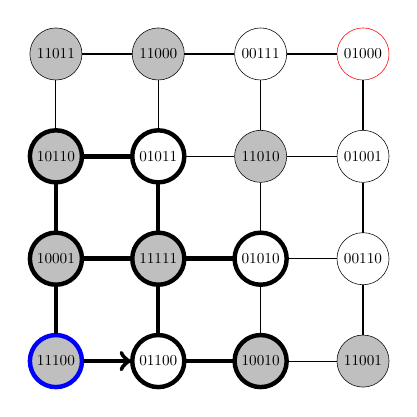
\begin{tikzpicture}
            \Bn[draw=blue] (n0) at (0,0) {11100};
            \Wn (n1) at (\coordscl{1}, \coordscl{0}) {01100};
            \Bn (n2) at (\coordscl{2}, \coordscl{0}) {10010};
            \bn (n3) at (\coordscl{3}, \coordscl{0}) {11001};
            \Bn (n4) at (\coordscl{0}, \coordscl{1}) {10001};
            \Bn (n5) at (\coordscl{1}, \coordscl{1}) {11111};
            \Wn (n6) at (\coordscl{2}, \coordscl{1}) {01010};
            \wn (n7) at (\coordscl{3}, \coordscl{1}) {00110};
            \Bn (n8) at (\coordscl{0}, \coordscl{2}) {10110};
            \Wn (n9) at (\coordscl{1}, \coordscl{2}) {01011};
            \bn (n10) at (\coordscl{2}, \coordscl{2}) {11010};
            \wn (n11) at (\coordscl{3}, \coordscl{2}) {01001};
            \bn (n12) at (\coordscl{0}, \coordscl{3}) {11011};
            \bn (n13) at (\coordscl{1}, \coordscl{3}) {11000};
            \wn (n14) at (\coordscl{2}, \coordscl{3}) {00111};
            \wn[draw=red] (n15) at (\coordscl{3}, \coordscl{3}) {01000};

            \draw[->,ultra thick]
                (n0) -- (n1);

            \draw[ultra thick]
                (n1) -- (n2)
                (n4) -- (n5)
                (n5) -- (n6)
                (n8) -- (n9)
                (n0) -- (n4)
                (n1) -- (n5)
                (n4) -- (n8)
                (n5) -- (n9)
                ;

            \draw
                (n2) -- (n3)
                (n6) -- (n7)
                (n9) -- (n10)
                (n10) -- (n11)
                (n12) -- (n13)
                (n13) -- (n14)
                (n14) -- (n15)
                (n2) -- (n6)
                (n3) -- (n7)
                (n6) -- (n10)
                (n7) -- (n11)
                (n8) -- (n12)
                (n9) -- (n13)
                (n10) -- (n14)
                (n11) -- (n15)
                ;

        \end{tikzpicture}

        \caption{Level 0}
        \label{fig:bmlrp-routing-l0}
    \end{subfigure}%
    %
    \begin{subfigure}[b]{0.23\textwidth}
        \centering

        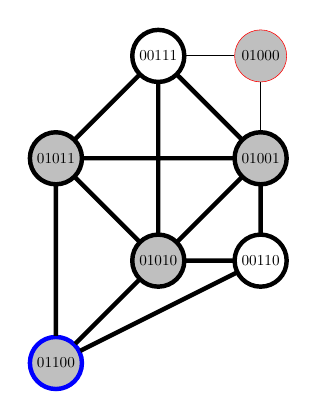
\begin{tikzpicture}
            \Bn[draw=blue] (n1) at (\coordscl{1}, \coordscl{0}) {01100};
            \Bn (n6) at (\coordscl{2}, \coordscl{1}) {01010};
            \Wn (n7) at (\coordscl{3}, \coordscl{1}) {00110};
            \Bn (n9) at (\coordscl{1}, \coordscl{2}) {01011};
            \Bn (n11) at (\coordscl{3}, \coordscl{2}) {01001};
            \Wn (n14) at (\coordscl{2}, \coordscl{3}) {00111};
            \bn[draw=red] (n15) at (\coordscl{3}, \coordscl{3}) {01000};

            \draw[ultra thick]
                (n1) -- (n6)
                (n1) -- (n7)
                (n1) -- (n9)
                (n6) -- (n7)
                (n6) -- (n9)
                (n6) -- (n11)
                (n6) -- (n14)
                (n7) -- (n11)
                (n9) -- (n11)
                (n9) -- (n14)
                (n9) -- (n11)
                (n11) -- (n14)
                ;

            \draw
                (n11) -- (n15)
                (n14) -- (n15)
                ;
        \end{tikzpicture}

        \caption{Level 1}
        \label{fig:bmlrp-routing-l1}
    \end{subfigure}%
    %
    \begin{subfigure}[b]{0.23\textwidth}
        \centering

        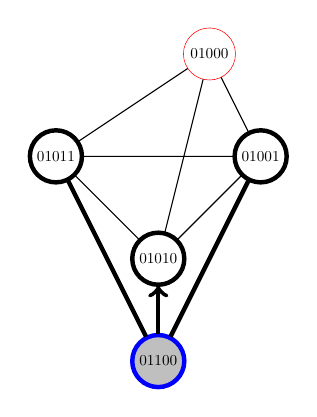
\begin{tikzpicture}
            \Bn[draw=blue] (n1) at (\coordscl{2}, \coordscl{0}) {01100};
            \Wn (n6) at (\coordscl{2}, \coordscl{1}) {01010};
            \Wn (n9) at (\coordscl{1}, \coordscl{2}) {01011};
            \Wn (n11) at (\coordscl{3}, \coordscl{2}) {01001};
            \wn[draw=red] (n15) at (\coordscl{2.5}, \coordscl{3}) {01000};

            \draw[->,ultra thick]
                (n1) -- (n6);

            \draw[ultra thick]
                (n1) -- (n9)
                (n1) -- (n11)
                ;

            \draw
                (n6) -- (n9)
                (n6) -- (n11)
                (n6) -- (n15)
                (n9) -- (n11)
                (n9) -- (n15)
                (n11) -- (n15)
                ;
        \end{tikzpicture}

        \caption{Level 2}
        \label{fig:bmlrp-routing-l2}
    \end{subfigure}%
    %
    \begin{subfigure}[b]{0.19\textwidth}
        \centering

        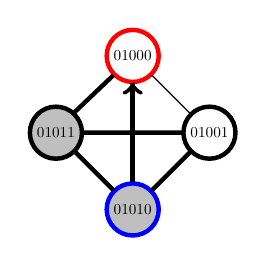
\begin{tikzpicture}
            \Bn[draw=blue] (n6) at (\coordscl{0.75}, \coordscl{0}) {01010};
            \Bn (n9) at (\coordscl{0}, \coordscl{0.75}) {01011};
            \Wn (n11) at (\coordscl{1.5}, \coordscl{0.75}) {01001};
            \Wn[draw=red] (n15) at (\coordscl{0.75}, \coordscl{1.5}) {01000};

            \draw[->,ultra thick]
                (n6) -- (n15);

            \draw[ultra thick]
                (n6) -- (n9)
                (n6) -- (n11)
                (n6) -- (n15)
                (n9) -- (n11)
                (n9) -- (n15)
                ;

            \draw
                (n11) -- (n15);

        \end{tikzpicture}

        \caption{Level 3}
        \label{fig:bmlrp-routing-l3}
    \end{subfigure}

    \caption{Routing in BMLRP}
    \label{fig:bmlrp-routing}
\end{figure}
